% 功能概述：保留本轮修订前的历史 ChEMBL 实验正文与表格；不与新闭库结果合并。
% 主要职责：归档不同样本批次的原报告；由 main.tex 的附录引入，来源见 main.before.tex。
\section{Historical QM9S--ChEMBL Evaluation}\label{sec:historical_results}
This appendix preserves the earlier manuscript results under their original protocol. They are not new JJ Test-200 measurements; all zero-exact claims below are restricted to this historical ChEMBL evaluation.


\begin{figure}[t]
\centering
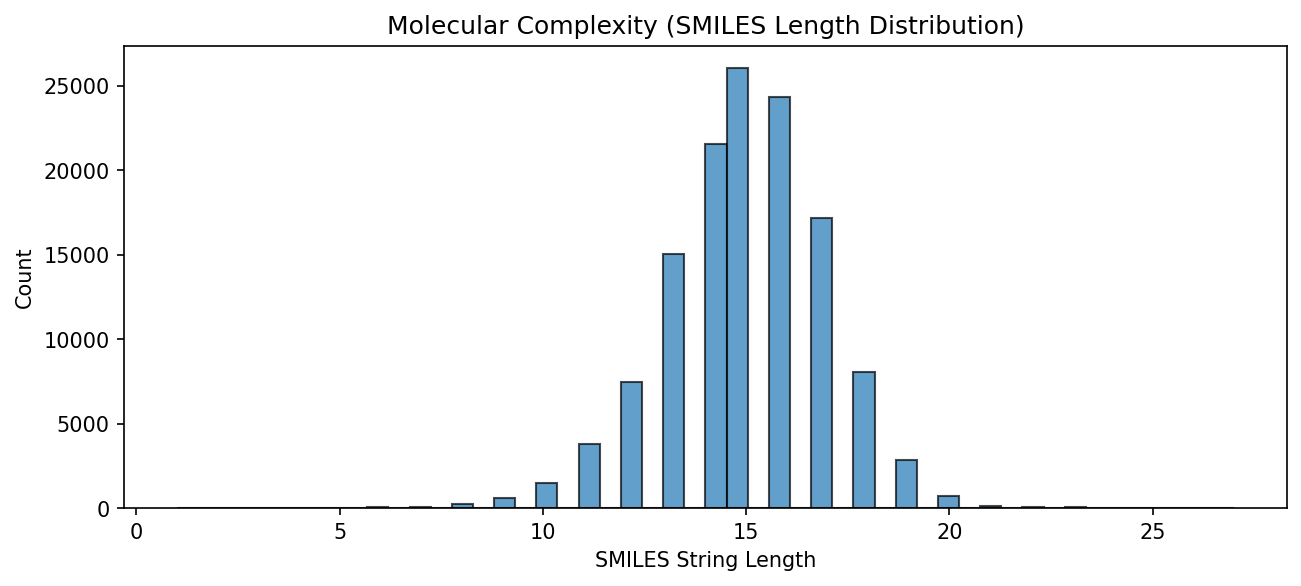
\includegraphics[width=.48\columnwidth]{figures/molecular_complexity.png}\hfill
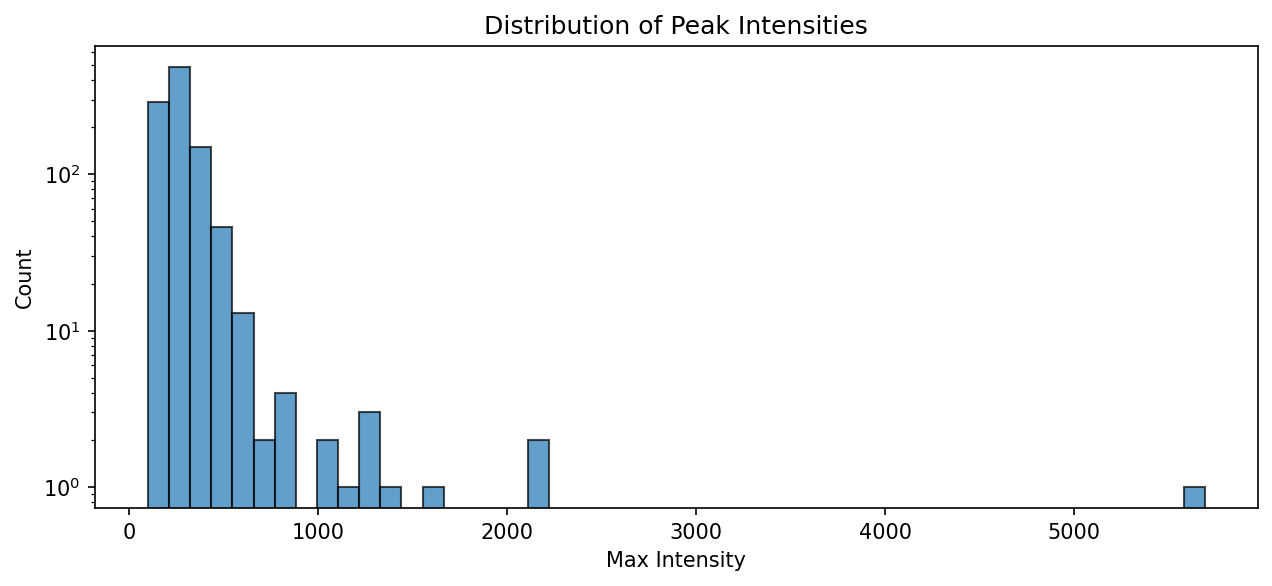
\includegraphics[width=.48\columnwidth]{figures/peak_intensity_distribution.png}
\caption{Statistical characteristics of the QM9S training dataset. Left: distribution of molecular complexity measured by SMILES sequence length, illustrating the structural diversity of molecules contained in the dataset. Right: distribution of maximum Raman peak intensities, showing substantial variation in spectral response strength across different molecular species.}
\label{fig:qm9s_statistics}
\end{figure}

\begin{figure}[t]
\centering
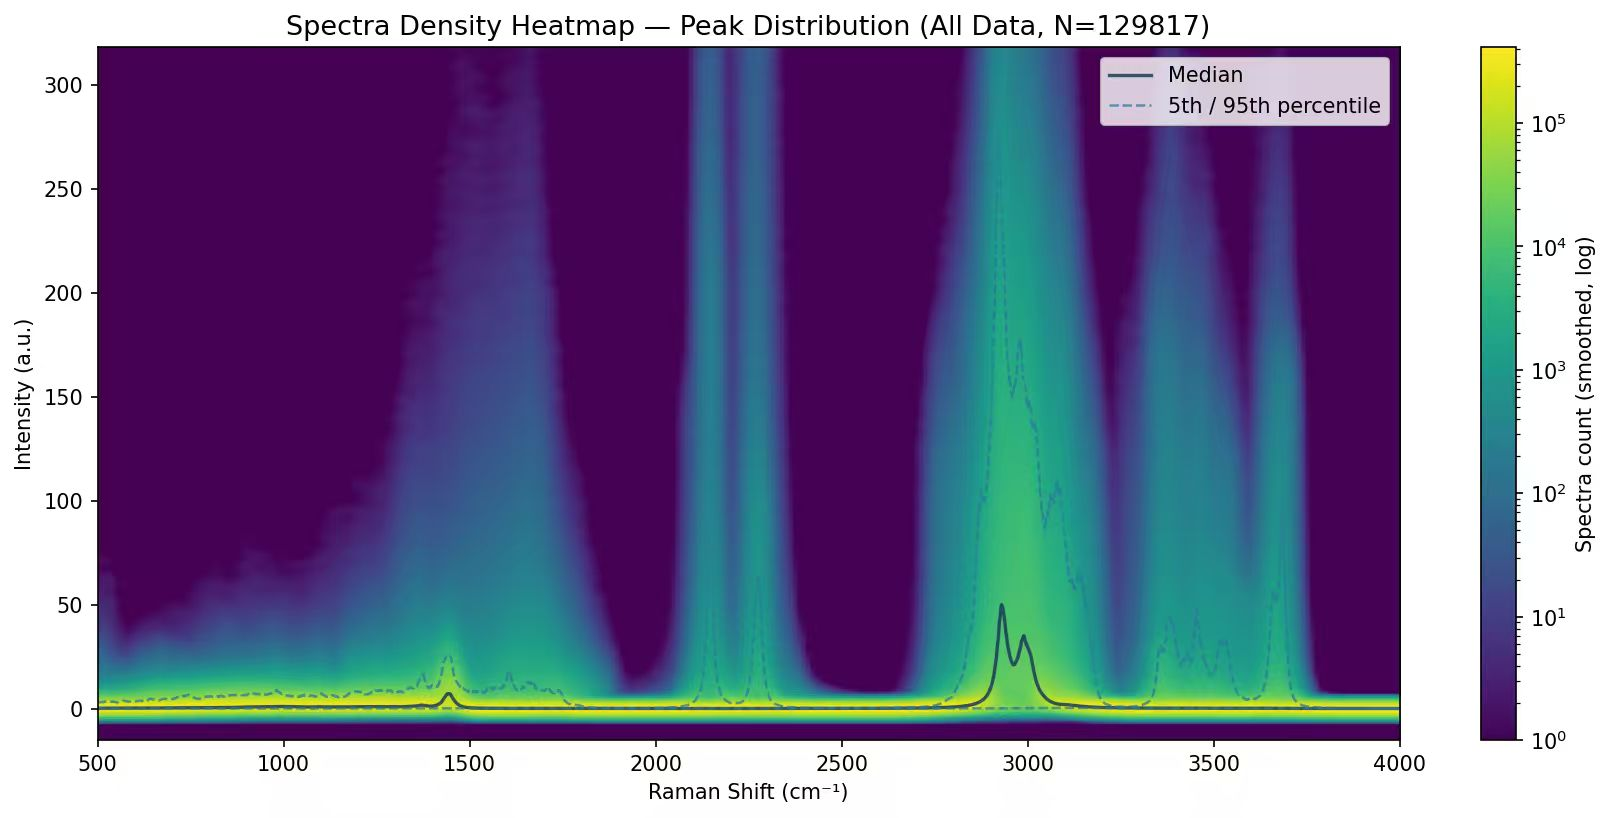
\includegraphics[width=\columnwidth]{figures/peak_distribution.jpg}
\caption{Two-dimensional density distribution of Raman spectra in the QM9S training set. The heatmap is generated by superimposing all spectra after normalization and resampling. High-density regions correspond to frequently occurring vibrational features, revealing the global spectral structure and characteristic Raman-active frequency bands present in the dataset.}
\label{fig:qm9s_heatmap}
\end{figure}

\subsection{Datasets and Benchmarks}

Evaluating Raman-based molecular identification requires both large-scale spectral data for representation learning and an independent benchmark for assessing generalization. To support reproducible applied evaluation, we employ two complementary datasets with separated roles: QM9S is used only to build the retrieval database and train the spectral encoder, whereas ChEMBL Raman spectra are reserved for out-of-domain testing.

\paragraph{QM9S Training Dataset.}

The retrieval model is trained using the QM9S dataset, a large-scale quantum chemistry database containing Raman spectra and molecular structures for over one hundred thousand organic molecules. Each sample consists of a molecular representation (SMILES) and a corresponding Raman spectrum represented on a uniform wavenumber grid spanning from 500 to 4000\,cm$^{-1}$ with a resolution of 1\,cm$^{-1}$. The resulting spectrum is therefore represented as a 3501-dimensional intensity vector. Figure~\ref{fig:qm9s_statistics} illustrates the distributions of molecular complexity and spectral intensity within the QM9S dataset.

The primary motivation for using QM9S is its scale and structural diversity. Since contrastive retrieval requires learning a semantically meaningful spectral embedding space, a large number of molecular examples is essential for capturing the relationship between spectral fingerprints and molecular structures. The resulting database serves as the retrieval corpus used in Stage~1 of SpectraExpert. The global spectral distribution of the dataset is visualized in Figure~\ref{fig:qm9s_heatmap}, where several high-density Raman-active regions can be observed.

\paragraph{ChEMBL Raman Evaluation Dataset.}

To evaluate the complete workflow, we adopt the Raman subset from \emph{A Dataset of Raman and Infrared Spectra as an Extension to the ChEMBL}~\cite{liang2025dataset}.

The ChEMBL Raman dataset is used exclusively for evaluation and shares no molecular overlap with the QM9S training set. Since the two datasets originate from distinct molecular collections, they exhibit substantially different structural distributions and spectral characteristics. Consequently, evaluation on the ChEMBL dataset provides a rigorous assessment of whether a Raman identification system can transfer from a curated quantum-chemistry corpus to larger, more application-oriented molecules.

This benchmark is intentionally harder than closed-library spectral search. A domain-specific tool with the exact target spectrum in its library would be expected to win by direct matching, but such a setting does not test molecular inference. Our evaluation instead asks whether a system trained and indexed on small QM9S molecules can provide useful candidate hypotheses, explanations, and edits for out-of-domain ChEMBL targets. This framing is central to the applied data-mining claim: the task measures transfer, retrieval quality, and evidence use under a controlled corpus shift.

\subsection{Experimental Setup}

We evaluate four categories of methods on the SpectraExpert SMILES-from-spectra prediction task. Retrieval methods (KNN, Encoder) retrieve the top-10 database candidates by spectral similarity across all 211 queries in the constructed ChEMBL test set. LLM Direct generates SMILES from spectral peak data alone on a randomly sampled 50-query batch from this test set. LLM Knowledge augments peak data with matched Nakamoto group-frequency rules and is evaluated on a 50-query batch randomly sampled from this test set. Agentic combines retrieval, Nakamoto rule matching, multi-step LLM reasoning, and a structural modification fallback, evaluated on a randomly sampled 20-query batch from the same test set. The LLM batches were sampled from the constructed evaluation set rather than selected by molecule length or difficulty; therefore, aggregate GED values across LLM settings should be interpreted as batch-level results unless the same query batch is used. Model-source citations are shown directly next to model names in the result tables.

Performance is measured by graph edit distance (GED; lower is better), Tanimoto similarity (higher is better), and the fraction of outputs yielding valid, parseable SMILES (Parsed). Generated SMILES are parsed and canonicalized before evaluation; invalid SMILES are excluded from GED and Tanimoto summaries and are instead counted through the Parsed metric. The reported $N$ denotes the number of attempted queries, not the number of valid outputs. GED is computed on molecular graphs after canonicalization using the same unit-cost edit model for all methods; atom labels and bond labels are retained, and implicit hydrogens are used consistently across predictions and ground truth. For retrieval methods, GED is the minimum across the top-10 candidates (best@10); for LLM and agentic methods it is computed from the single predicted SMILES. Exact match denotes equality after molecular-graph canonicalization.

\subsection{Main Results}

Full results are reported in Table~\ref{tab:main_results}. No method achieves any exact matches, reflecting the fundamental difficulty of this cross-domain task (retrieval database: QM9S, $\leq9$ heavy atoms; test set: ChEMBL, up to 21 heavy atoms). The table is placed at the beginning of the Results section to make the complete experimental picture explicit: retrieval baselines, direct LLM generation, knowledge-augmented prompting, and the full agentic pipeline are all reported with GED, median GED, variance, sample count, and parse rate.

The strongest numbers should be interpreted cautiously. The LLM Knowledge row for o3 achieves the lowest valid-only GED on its sampled batch, but it does not use the same query set as the retrieval rows. Conversely, retrieval is evaluated on all 211 queries and therefore provides the most stable estimate of benchmark difficulty. The practical conclusion is not that one LLM universally solves the task, but that rule-grounded prompts can sometimes produce strong hypotheses while structured-output failures and batch variation remain major limitations.

\begin{table*}[t]
\centering
\PaperTableSetup{\small}
\caption{Historical QM9S--ChEMBL results across methods and models}
\label{tab:main_results}
\begin{tabularx}{\linewidth}{l>{\raggedright\arraybackslash}Xrrrrr}
\toprule
\rowcolor{HdrBg}
\multicolumn{1}{l}{\PaperHead{Method}} & \multicolumn{1}{l}{\PaperHead{Model}} & \PaperHead{GED$_\mu$} & \PaperHead{GED$_{50}$} & \PaperHead{GED$_\sigma$} & \PaperHead{$N$} & \PaperHead{Parsed}\\[1pt]
\midrule
\PaperGroup{7}{RetBg}{Retrieval}
\rowcolor{RetBg!55}
Encoder & N/A & 16.93 & 17.0 & 4.63 & 211 & 1.00\\
\rowcolor{RetBg!28}
KNN & N/A & 17.04 & 17.0 & 3.91 & 211 & 1.00\\
\PaperGroup{7}{DirBg}{LLM Direct}
\rowcolor{DirBg!55}
LLM-Direct & GPT-5~\cite{gpt-5}$^\dagger$ & 22.79 & 22.0 & 4.22 & 50 & 0.38\\
\rowcolor{DirBg!28}
LLM-Direct & o3~\cite{o3_and_o4-mini} & 23.53 & 24.0 & 4.38 & 50 & 0.94\\
\rowcolor{DirBg!55}
LLM-Direct & Claude-Sonnet-4-6~\cite{claude-sonnet-4-6} & 23.82 & 24.0 & 4.57 & 50 & 1.00\\
\rowcolor{DirBg!28}
LLM-Direct & Gemini-2.5-Flash~\cite{gemini2-5}$^\dagger$ & 23.90 & 24.5 & 5.49 & 50 & 0.20\\
\rowcolor{DirBg!55}
LLM-Direct & DeepSeek-v4-Flash~\cite{deepseek2026deepseek}$^\dagger$ & 24.68 & 26.0 & 5.27 & 50 & 0.44\\
\PaperGroup{7}{KnwBg}{LLM Knowledge}
\rowcolor{KnwBg!55}
LLM-Know. & o3~\cite{o3_and_o4-mini} & 13.52 & 14.0 & 5.95 & 50 & 0.84\\
\rowcolor{KnwBg!28}
LLM-Know. & GPT-5~\cite{gpt-5}$^\dagger$ & 14.86 & 16.0 & 5.60 & 50 & 0.42\\
\rowcolor{KnwBg!55}
LLM-Know. & DeepSeek-v4-Flash~\cite{deepseek2026deepseek} & 15.24 & 15.0 & 6.28 & 50 & 0.68\\
\rowcolor{KnwBg!28}
LLM-Know. & Claude-Sonnet-4-6~\cite{claude-sonnet-4-6} & 16.90 & 16.5 & 13.92 & 50 & 0.96\\
\rowcolor{KnwBg!55}
LLM-Know. & Gemini-2.5-Flash~\cite{gemini2-5}$^\dagger$ & 17.70 & 16.5 & 7.00 & 50 & 0.20\\
\PaperGroup{7}{AgtBg}{Agentic}
\rowcolor{AgtBg!55}
Agentic & Gemini-2.5-Flash~\cite{gemini2-5} & 15.67 & 15.0 & 5.03 & 20 & 1.00\\
\rowcolor{AgtBg!28}
Agentic & DeepSeek-v4-Flash~\cite{deepseek2026deepseek} & 15.73 & 17.0 & 3.86 & 20 & 0.85\\
\rowcolor{AgtBg!55}
Agentic & Claude-Sonnet-4-6~\cite{claude-sonnet-4-6} & 16.16 & 15.0 & 4.91 & 20 & 1.00\\
\rowcolor{AgtBg!28}
Agentic & o3~\cite{o3_and_o4-mini} & 18.07 & 18.0 & 5.15 & 20 & 0.95\\
\rowcolor{AgtBg!55}
Agentic & GPT-5~\cite{gpt-5}$^\ddagger$ & 21.00 & 21.0 & 0.00 & 20 & 0.05\\
\bottomrule
\end{tabularx}
\arrayrulecolor{black}
\PaperNote{GED$_\mu$, GED$_{50}$, GED$_\sigma$: mean, median and standard deviation. Parsed: valid-SMILES fraction. $^\dagger$Parse rate below 0.50; GED uses valid outputs only. $^\ddagger$Near-zero parse rate; result not meaningful. Retrieval uses all 211 queries; Direct and Knowledge use randomly sampled batches of 50; Agentic uses 20. Batches differ by method.}
\end{table*}

\subsection{Retrieval Baselines: Encoder vs.\ KNN}

The encoder and KNN retrieval methods perform virtually identically. GED means differ by only 0.11 (16.93 vs.\ 17.04), within noise. The encoder is faster (14.9\,s end-to-end), making it the preferable baseline for downstream comparisons.

\subsection{LLM Direct and LLM Knowledge}

LLM Direct and LLM Knowledge are evaluated on randomly sampled 50-query batches from the same constructed ChEMBL test set. Raw GED values should be interpreted as setting-specific batch summaries; strict paired comparisons require the same query list.

Table~\ref{tab:paired_direct} provides a batch-controlled comparison by evaluating retrieval baselines on the same randomly sampled queries used for LLM Direct. LLM Direct achieves GED values from 22.79 to 24.68, bracketing the retrieval top-1 (Encoder: 24.48) but falling slightly short of the Encoder best@10 oracle (21.98). This confirms that LLMs can leverage functional-group knowledge to propose plausible structures without any database, yet cannot yet surpass a well-tuned retrieval re-ranker on this sampled cross-domain batch.

On the randomly sampled LLM Knowledge batch, o3 achieves GED 13.52 (Table~\ref{tab:main_results}), showing that Nakamoto rule augmentation can produce strong valid-only predictions on sampled ChEMBL queries. Parse rate remains a key differentiator: Claude-Sonnet achieves 96\% compliance with knowledge-augmented prompts vs.\ 20\% for Gemini-2.5-Flash. The counterintuitive Tanimoto result for Gemini (0.000) in LLM Knowledge mode indicates systematic hallucination: its parsed SMILES bear no fingerprint overlap with ground truth despite non-trivial GED values.

\begin{table}[t]
\centering
\PaperTableSetup{\footnotesize}
\caption{Historical comparison on the paired Direct batch}
\label{tab:paired_direct}
\begin{tabularx}{\linewidth}{>{\raggedright\arraybackslash}Xrr}
\toprule
\rowcolor{HdrBg}
\multicolumn{1}{l}{\PaperHead{Method}} & \PaperHead{GED$_\mu$} & \PaperHead{Tanimoto}\\[1pt]
\midrule
\PaperGroup{3}{DirBg}{Direct generation}
\rowcolor{DirBg!55}
LLM-Direct GPT-5~\cite{gpt-5} & 22.79 & 0.125\\
\rowcolor{DirBg!28}
LLM-Direct o3~\cite{o3_and_o4-mini} & 23.53 & 0.114\\
\rowcolor{DirBg!55}
LLM-Direct Claude-S-4.6~\cite{claude-sonnet-4-6} & 23.82 & 0.117\\
\PaperGroup{3}{RetBg}{Retrieval top-1}
\rowcolor{RetBg!55}
Encoder top-1 & 24.48 & 0.058\\
\rowcolor{RetBg!28}
KNN top-1 & 25.92 & 0.061\\
\PaperGroup{3}{RetBg}{Retrieval best@10 oracle}
\rowcolor{RetBg!55}
Encoder best@10 & 21.98 & --\\
\rowcolor{RetBg!28}
KNN best@10 & 22.00 & --\\
\bottomrule
\end{tabularx}
\arrayrulecolor{black}
\PaperNote{All methods use the same 50 randomly sampled ChEMBL queries. GED uses valid predictions. Best@10 is a GED oracle, so its Tanimoto is omitted.}
\end{table}

\subsection{SMILES Output Validity}

Parse rates vary substantially across models (Table~\ref{tab:parsing}). Claude-Sonnet-4-6 achieves perfect compliance in direct and agentic modes, whereas Gemini-2.5-Flash fails frequently in unstructured settings. The agentic schema improves Gemini validity (0.20 $\rightarrow$ 1.00) but degrades GPT-5 (0.38 $\rightarrow$ 0.05), confirming that parseability is a necessary interface requirement rather than a standalone measure of chemical accuracy.

\begin{table}[t]
\centering
\PaperTableSetup{\footnotesize}
\caption{Historical structured-output validity by model}
\label{tab:parsing}
\begin{tabularx}{\linewidth}{>{\raggedright\arraybackslash}Xrrr}
\toprule
\rowcolor{HdrBg}
\multicolumn{1}{l}{\PaperHead{Model}} & \PaperHead{Direct} & \PaperHead{Knowledge} & \PaperHead{Agentic}\\[1pt]
\midrule
\rowcolor{DirBg!55}
Claude-Sonnet-4-6~\cite{claude-sonnet-4-6} & 1.00 & 0.96 & 1.00\\
\rowcolor{DirBg!28}
o3~\cite{o3_and_o4-mini} & 0.94 & 0.84 & 0.95\\
\rowcolor{DirBg!55}
DeepSeek-v4-Flash~\cite{deepseek2026deepseek} & 0.44 & 0.68 & 0.85\\
\rowcolor{DirBg!28}
GPT-5~\cite{gpt-5} & 0.38 & 0.42 & 0.05\\
\rowcolor{DirBg!55}
Gemini-2.5-Flash~\cite{gemini2-5} & 0.20 & 0.20 & 1.00\\
\bottomrule
\end{tabularx}
\arrayrulecolor{black}
\PaperNote{Fraction of predictions yielding valid, parseable SMILES; higher is better.}
\end{table}

\subsection{Agentic Pipeline}

On the sampled 20-query agentic batch, the full pipeline includes individual predictions with GED as low as 8.0 for Claude, DeepSeek, and o3, showing that reasoning can succeed when retrieval supplies a structurally proximate candidate. Table~\ref{tab:agentic_decisions} shows that SELECTED decisions consistently outperform MODIFIED decisions; the fallback is mainly triggered when the QM9S--ChEMBL domain gap leaves all retrieved candidates structurally distant. Gemini always invokes MODIFY, while GPT-5 is mostly UNCERTAIN in multi-turn use.

A notable negative result is that modification degrades average GED relative to the SELECT path ($+4.86$ for Claude, $+2.98$ for DeepSeek, $+1.23$ for o3), because unconstrained SMILES editing from a poor starting point is itself hard. This highlights the need for calibrated handoffs and chemistry-aware constrained editing in future retrieval-augmented scientific workflows.

\begin{table}[t]
\centering
\PaperTableSetup{\fontsize{7.5}{9}\selectfont}
\caption{Historical agentic decision breakdown}
\label{tab:agentic_decisions}
\begin{tabularx}{\linewidth}{>{\raggedright\arraybackslash}Xrrrr}
\toprule
\rowcolor{HdrBg}
\multicolumn{1}{l}{\PaperHead{Model}} & \PaperHead{\shortstack{SELECT\\($n$)}} & \PaperHead{GED} & \PaperHead{\shortstack{MODIFY\\($n$)}} & \PaperHead{GED}\\[1pt]
\midrule
\rowcolor{AgtBg!55}
Claude-Sonnet-4-6~\cite{claude-sonnet-4-6} & 6 & 12.8 & 14 & 17.7\\
\rowcolor{AgtBg!28}
DeepSeek-v4-Flash~\cite{deepseek2026deepseek} & 7 & 14.1 & 10 & 17.1\\
\rowcolor{AgtBg!55}
o3~\cite{o3_and_o4-mini} & 6 & 17.3 & 13 & 18.6\\
\rowcolor{AgtBg!28}
Gemini-2.5-Flash~\cite{gemini2-5} & 0 & N/A & 20 & 15.7\\
\rowcolor{AgtBg!55}
GPT-5~\cite{gpt-5} & 0 & N/A & 1 & N/A\\
\bottomrule
\end{tabularx}
\arrayrulecolor{black}
\PaperNote{20 attempted queries per model. GED is computed on valid predictions only.}
\end{table}

\subsection{Summary and Practical Recommendations}

Across all settings, retrieval is the most stable baseline: the encoder achieves mean best@10 GED 16.93 over all 211 queries, and retrieval best@10 remains lower than every direct LLM result on the paired direct batch. LLMs add complementary capabilities rather than replacing retrieval: direct prompting gives zero-shot structures, Nakamoto-rule prompting improves valid-only predictions on sampled batches, and the agentic pipeline provides interpretable rule-grounded traces with individual GED values as low as 8.0. For deployment, Claude Sonnet 4.6 is preferred for structured-output reliability, while o3 gives the best LLM+KB GED on its sampled batch. Overall, SpectraExpert should be read as a benchmarked applied workflow that decomposes a difficult inverse problem into measurable retrieval, rule-matching, and reasoning components under domain shift.

